\chapter{Otras Señales}
Se conectaron al analizador de espectros las siguientes
señales con amplitud $250\si{\milli\volt}pp$ y a frecuencia
$125\si{\kilo\hertz}$ y máxima.

\begin{enumerate}
    \item $\sin(x)/x$
    \item Tren de Pulsos (Tren de Pulsos con DC mínimo)
\end{enumerate}

\section{$\sin(x)/x$}
\begin{figure}[ht]
    \begin{center}
        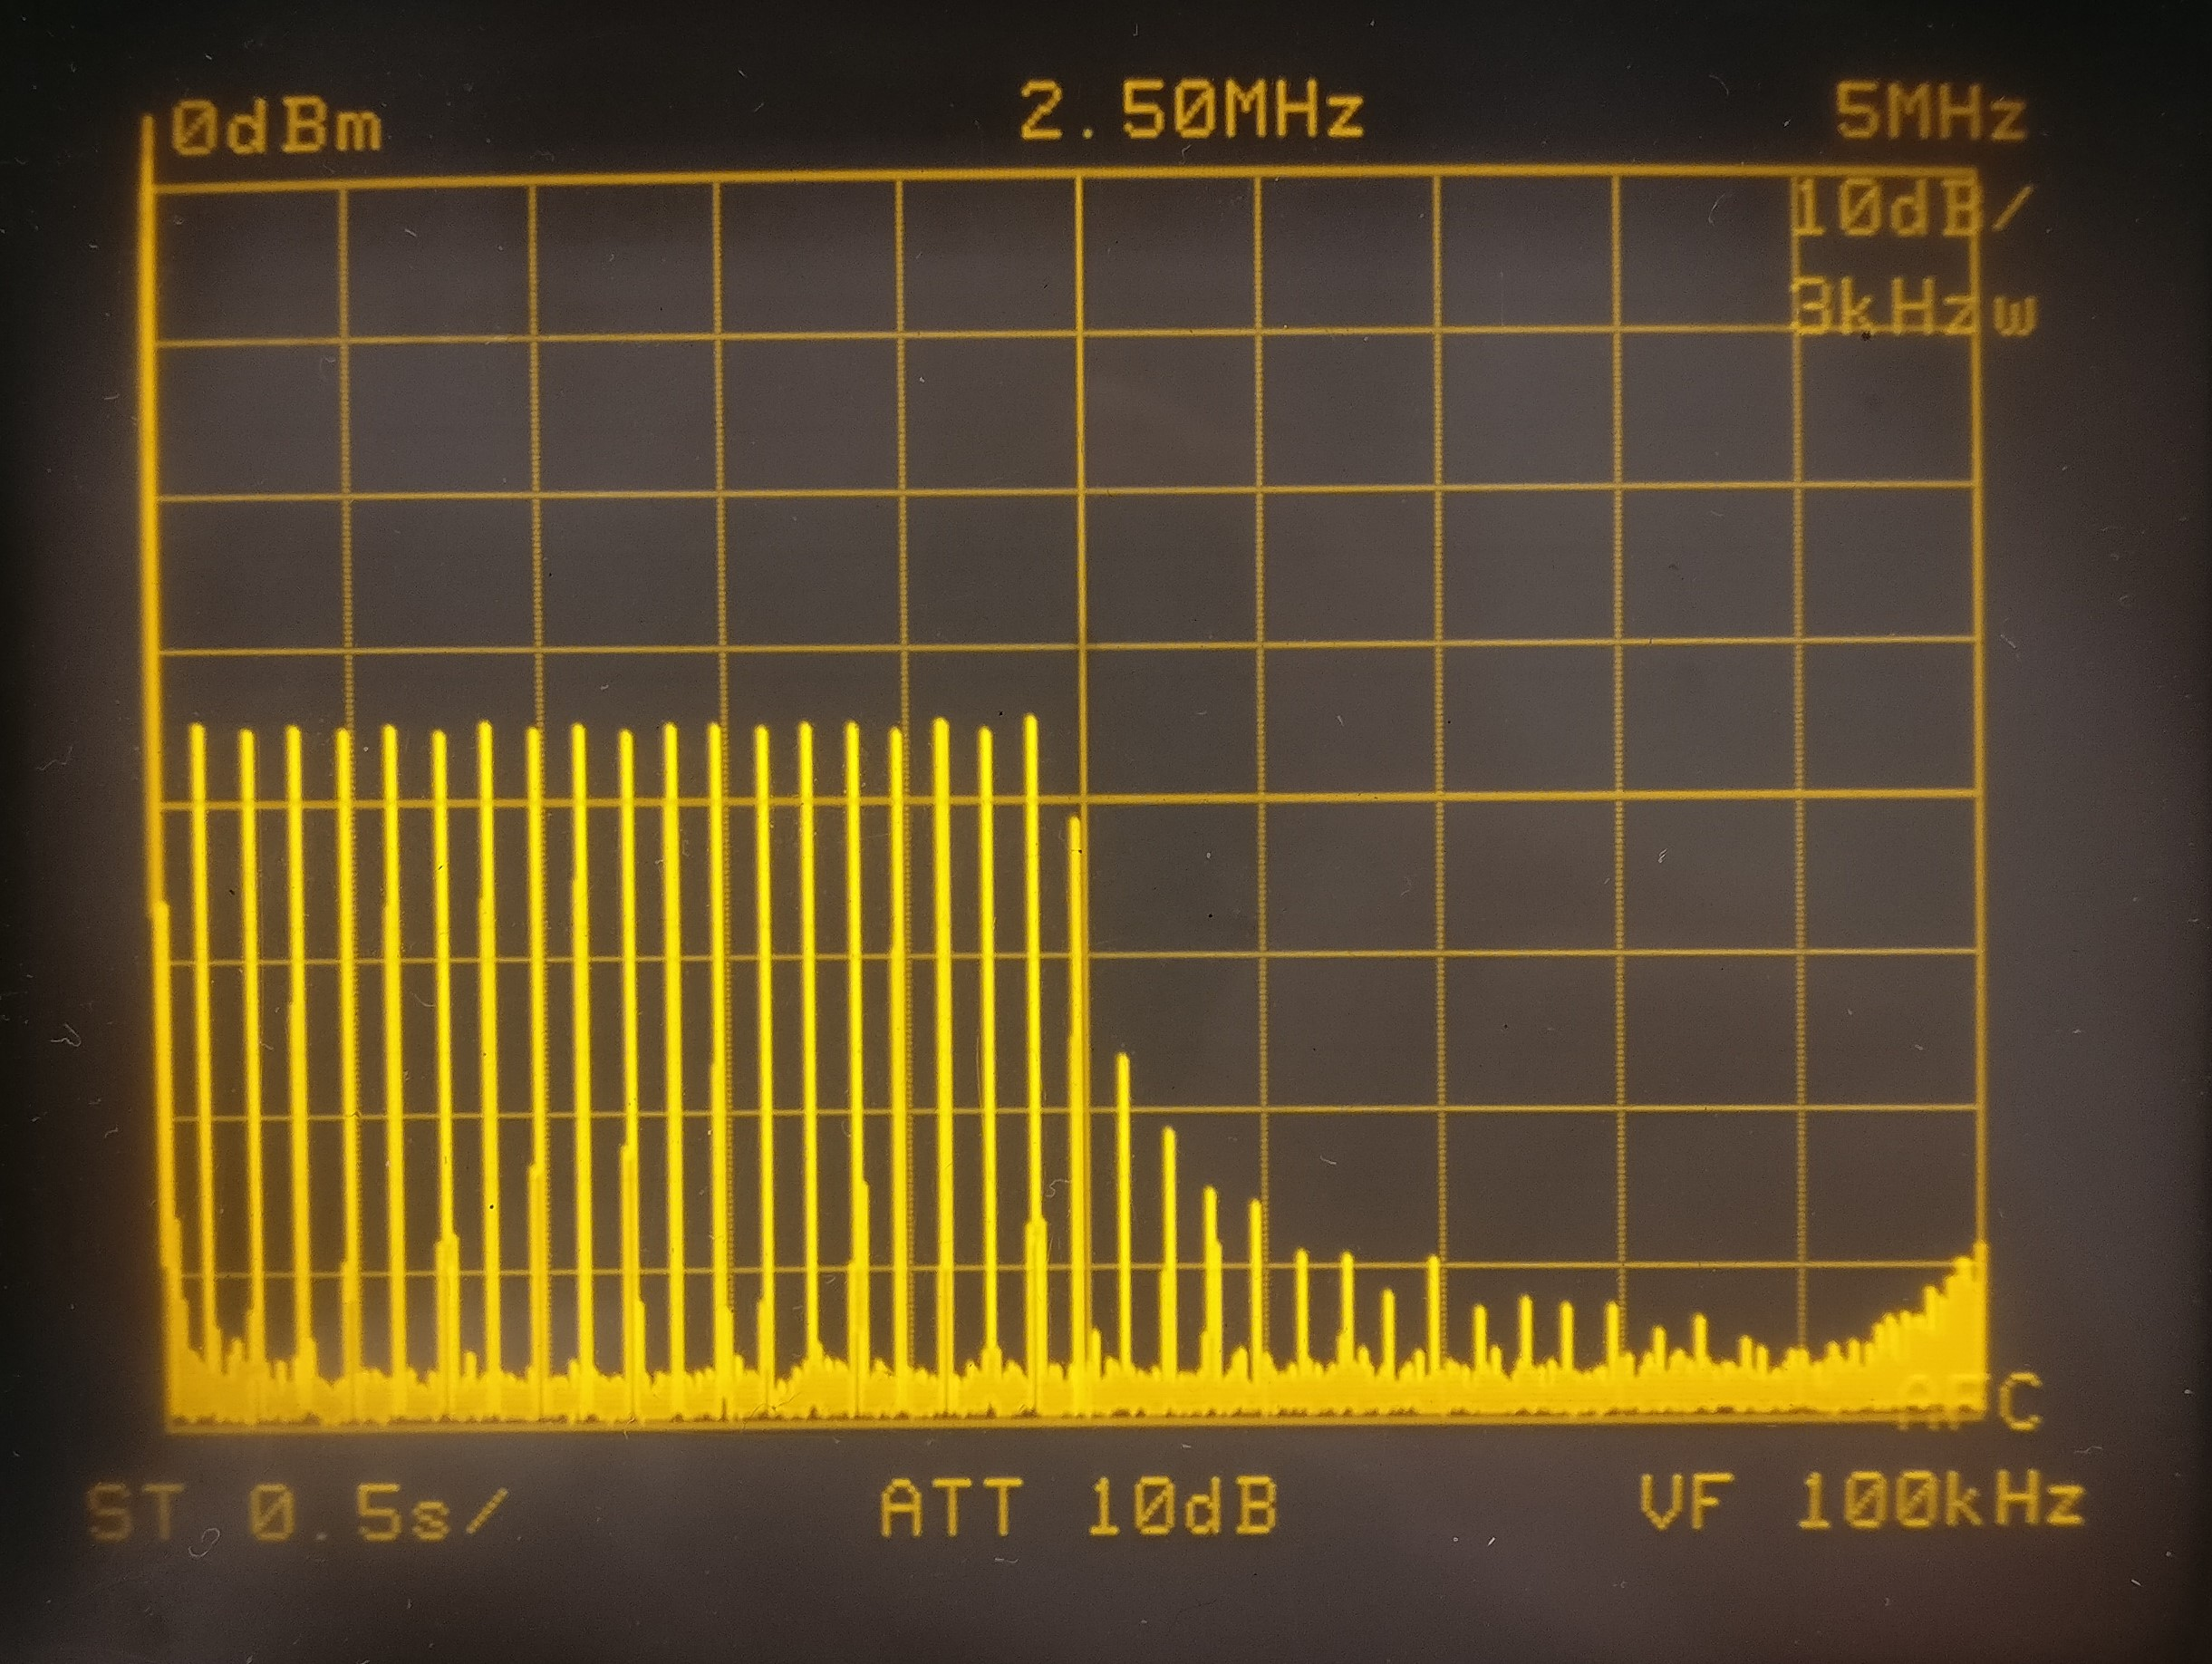
\includegraphics[width=0.6\linewidth]{contenido/img/espectro_sinx.jpg}
        \caption{Espectro de la señal de la función}
        \label{fig:espectro_sin}
    \end{center}
\end{figure}

\newpage
\section{Tren de Pulsos}

\begin{figure}[ht]
    \begin{center}
        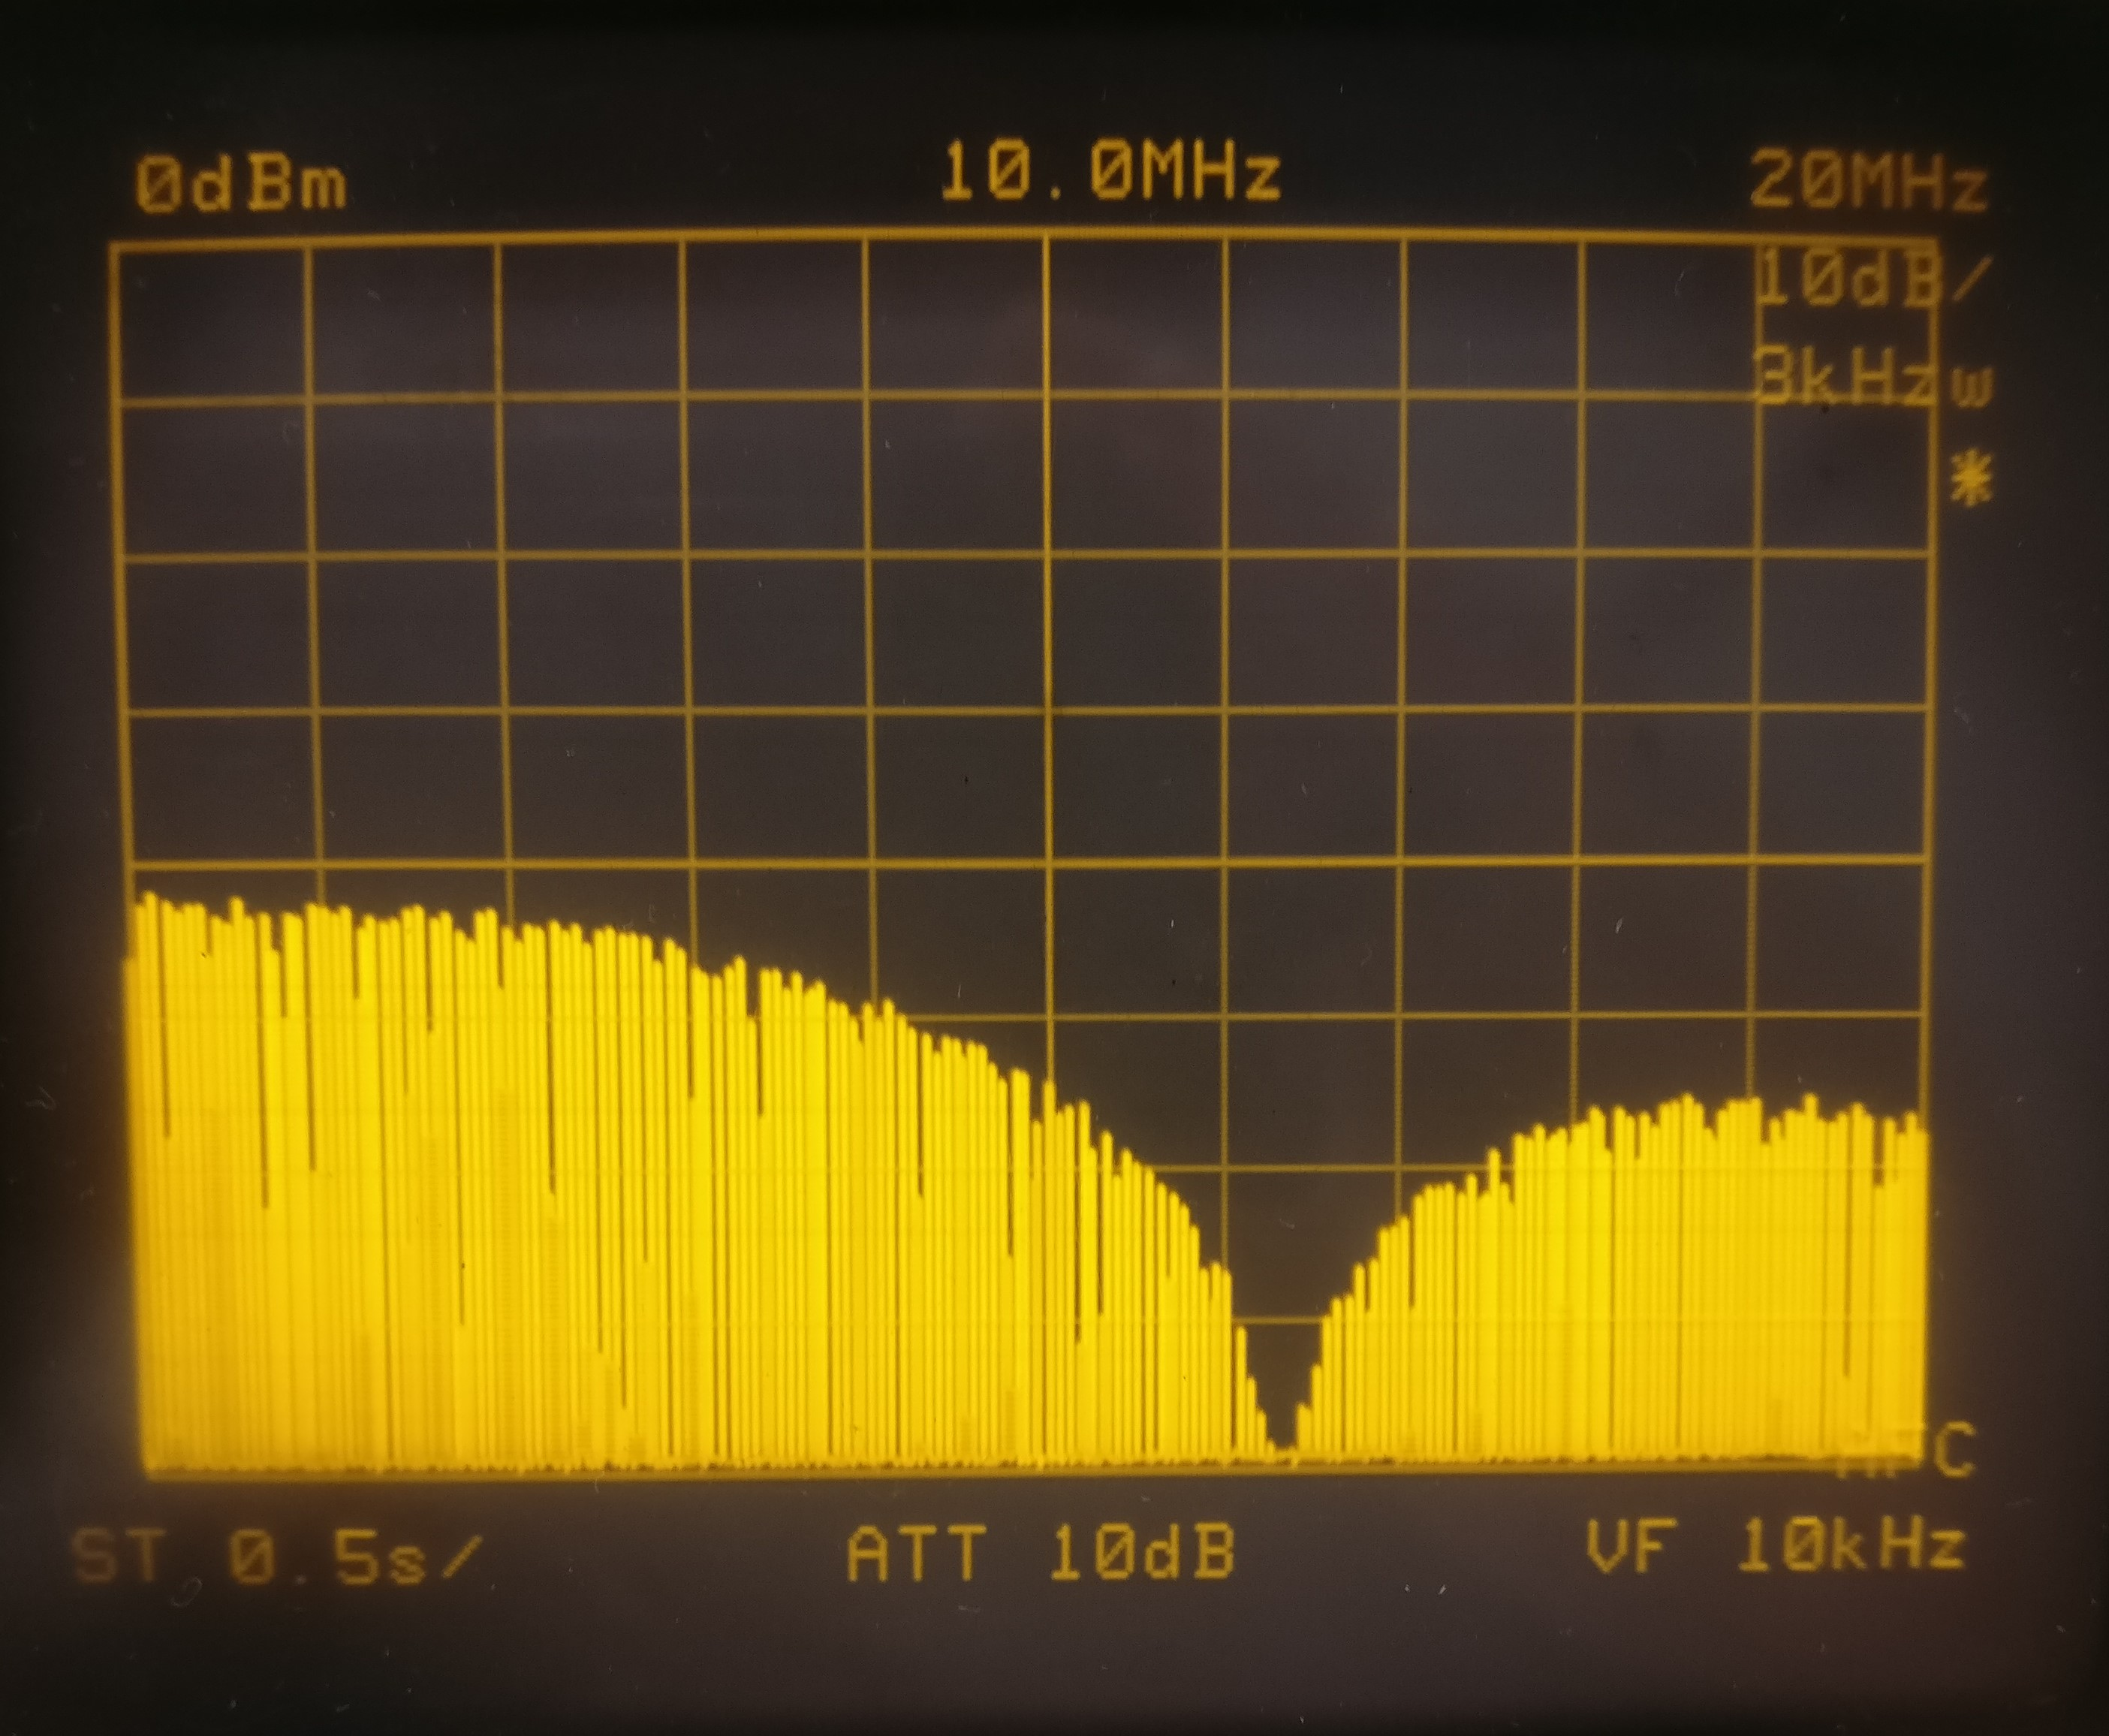
\includegraphics[width=0.6\linewidth]{contenido/img/espectro_dc01.jpg}
        \caption{Espectro del Tren de Pulsos con DC = 1\%}
         \label{fig:espectro_tren}
    \end{center}
\end{figure}

Es de esperarse para esta señal que, en lo que parece ser el armónico 100 (figura \ref{fig:espectro_tren}), este 
tiene una potencia casi nula comparada a la de los otros armónicos, dado que tiene un DC de 1\%.